\chapter{Stand der Technik}
<<<<<<< HEAD


\section{Synchronmaschine mit Dauermagneterregung}
\subsection{Auswertung der Anrtiebswelle}

\section{Curtis Controller}
\subsection{Allgemeines}
\subsection{VCL}
\subsection{Feldorientierte Regelung}

\section{Leonard-Umformer}
\subsection{Allgemeines}
\subsection{ }

\section{KPI-Regler}
\subsection{Allgemeines}
\subsection{ }
=======
\section{Steuereinheiten}
\section{Bussysteme}
<<<<<<< Updated upstream
>>>>>>> 909ce2e364172eacda8c0ef77d3e60d4f81ec294
=======

\newpage

\section{Kühlung} 

Bei dem Vorgang der Kühlung oder Abkühlung, wird einem System Wärme, oder thermische Energie entzogen. (Deshalb auch Entwärmung genannt)
Unter Kühlung versteht man die Übertragung von Wärme einer technischen Komponente, an die Umwelt. Dieses Phänomen wird oft beabsichtigt hervorgerufen, um bestimmte temperaturabhängige Eigenschaften erreichen und erhalten, aber auch Systeme vor Überhitzung schützen zu können. 
Durch Isolierungen, wie beispielsweise bei Häusern, kann unerwünschter Wärmeentzug zu einem gewissen Teil verhindert werden.



\subsection{Thermodynamische Grundlagen}

Der Entzug von Wärme geht bei Feststoffen und Flüssigkeiten durch Wärmeübertragung entsprechend einem Temperaturgradienten vonstatten. Die wesentlichen Prozesse sind dabei Wärmeleitung und Wärmestrahlung, eingeschränkt auch die Konvektion. Da all diese Prozesse spontan ablaufen und folglich entsprechend den Grundgesetzen der Thermodynamik einen Temperaturausgleich zur Folge haben, kann eine künstlich erwünschte Kühlung eines Gegenstandes gegen einen Temperaturgradienten nur unter hohem Energieaufwand erfolgen. 

Insgesamt wird dies jedoch immer mit einer Erhöhung der Gesamtentropie und damit im Regelfall einer Umwandlung Energieformen höherer Ordnung in thermische Energie resultieren. Eine Kühlung im Sinne einer Reduzierung der thermischen Energie eines abgeschlossenen Systems ist daher nicht möglich, was sich in der Praxis zum Beispiel darin äußert, dass auch Kühlschränke letztlich die Temperatur (der Umgebung) erhöhen und nicht senken, wenn dies auch lokal der Fall sein mag.

Die entscheidenden Einflussfaktoren sind dabei durch Wärmeleitkoeffizient, Wärmeübergangskoeffizient und Wärmekapazität gegeben. Bei Flüssigkeiten spielt die Wärmeleitung und Wärmestrahlung ebenfalls eine Rolle, hinzu kommt jedoch die Konvektion als wesentlicher Prozess des Temperaturausgleichs. Dieser dominiert hingegen bei Gasen, wobei diese allgemein nur sehr schlecht über Prozesse der Wärmeleitung abkühlen. Sie unterliegen jedoch verschiedenen Gasgesetzen, wodurch vor allem der adiabatischen Abkühlung und dem Joule-Thomson-Effekt eine große Rolle zukommt. 

\newpage

\subsection{Technische Anwendung}

Kühlsysteme können nach dem verwendeten Wärmeträgermedium unterteilt werden. Die geläufigsten Arten der Kühlung sind:

\begin{itemize}
	\item Wasserkühlung und
	\item Luftkühlung.
	\item Ölkühlung z.  B. im Automotor und in Hydrauliksystemen (hydraulischen Antrieben) 
	\item Natriumkühlung in Kernkraftwerken
	\item Kühlung durch Peltier-Elemente Kühlung von Prozessoren
\end{itemize}

\subsection{Funktionsweise}

Eine Kühlung basiert meist auf der Übertragung der Wärme (Wärmeleitung) vom zu kühlendem Körper zum Kühlstoff (Gas oder Flüssigkeit) und deren Abtransport (Wärmeströmung).
Bei manchen Anwendungen mit engen Platzverhältnissen (innerhalb eines Computers oder HiFi-Verstärkers) werden zum Abtransport Heatpipes verwendet.
Bei den meisten Motoren wird eine spezielle Kühlflüssigkeit eingesetzt.

\subsection{Einsatzgebiete}

Kühlungen werden in fast allen technischen Geräten, die sich erwärmen, eingesetzt. Zumeist wird jedoch eine passive Kühlung, das heißt die Abgabe der Wärme über Kühlkörper an die umgebende Luft, genutzt.
Das bekannteste Beispiel ist der Kühlschrank zur Konservierung von Lebensmitteln. In Kfz wird meist eine Wasserkühlung benutzt, in Computern kommen überwiegend Luftkühlungen zum Einsatz. Ein weiteres großes Einsatzgebiet ist zum Beispiel die Klimaanlage.

\subsection{Beispiele}

\begin{itemize}
	\item Kühlsysteme von Kraftwerken und chemischen Prozessen
	\item Kühlung in der Klimatechnik
	\item Öl- und Ladeluftkühler im Turbodiesel-Motor
	\item Abgaskühlung in AGR-Systemen (zur Emissionsreduzierung (NOx))
	\item Wasserkühlung eines Automotors
	\item Luftkühlung eines Prozessors
\end{itemize}

%Quelle: https://www.chemie.de/lexikon/K%C3%BChlung.html 09:29 Uhr 17.03.2021
%Dieser Artikel basiert auf dem Artikel Kühlung aus der freien Enzyklopädie Wikipedia und steht unter der GNU-Lizenz für freie Dokumentation. In der Wikipedia ist eine Liste der Autoren verfügbar.

Zu Kühlung siehe auch \cite{Kuehlung1,Kuehlung2}

\newpage

\subsection{Wasserkühlung} 

Bei einer Wasserkühlung (Flüssigkeitskühlung), wird Wasser als primäres Kühlmittel verwendet wird. Die Wasserkühlung kann sehr vielseitig eingesetzt werden. Wasser wird als Kühlung in Elektro- wie auch in Verbrennungsmotoren, Hochöfen, Stromrichtern, Kraftwerken, Computern und noch vielen weiteren Anwendungen verwendet.   

\subsubsection{Wasserkühlung bei elektronischen Geräten}

Seit 1930 werden die röhrenbestückten Endstufen von Hochleistungssendern mit Wasser gekühlt. Da hierbei hohe elektrische Spannungen zum Einsatz kommen, kann nur destilliertes deionisiertes Wasser zum Einsatz kommen. Dieses gibt in einem Wärmeübertrager seine Wärme an einem zweiten Kreislauf ab, in dem das Wasser keinen besonderen Reinheitsanforderungen genügen muss, da es mit keinen spannungsführenden Komponenten in Kontakt kommt.

Bei Hochleistungsröhren wird die Siedekondensationskühlung angewandt. Bei dieser Technik sind Dampferzeugung und Kondensation räumlich nicht voneinander getrennt. Das Kühlmittel durchfließt den Kühlkanal, der mit zur Anodeninnenseite hin orientierten Nuten ausgestattet ist. Der in diesen Nuten entstehende Dampf gerät in den Hauptkühlkanal, wo er verwirbelt wird und wieder kondensiert. Da sich dieser Vorgang bei Temperaturen von über 100 °C abspielt, und den Aggregatzustand flüssig zu gasförmig nutzt, können mit diesem Kühlverfahren auf Grund der dafür notwendigen Verdampfungswärme auch bei relativ kleinen Röhren große Wärmemengen abgeführt werden.
Moderne, halbleiterbestückte Sender haben keine Wasserkühlung mehr.
Wasserkühlung wird auch in der Leistungselektronik angewandt. Zum Beispiel für Stromrichter in Anlagen der Hochspannungs-Gleichstrom-Übertragung oder für Traktionsstromrichter in Schienenfahrzeugen.


\subsubsection{Wasserkühlung in Personal Computern}

Wasserkühlungen werden auch in modernen PC-Systemen zur leisen und effektiven Kühlung einzelner Komponenten eingesetzt. Dabei wird am häufigsten der Hauptprozessor gekühlt. Weitere Komponenten, die in den Kühlkreislauf eingebunden werden können, sind Grafikkarten, Hauptplatinen­chipsätze, Festplatten, Netzteile, Spannungswandler und auch RAM-Bausteine.
Wasserkühlungen für PCs sind in PC-Moddingkreisen sehr verbreitet. Mittlerweile ist ein großer Markt um Wasserkühlungen entstanden.
Die Vorteile einer Wasserkühlung sind zum einen die effektive Kühlung der Hardware mit für Modder und Overclocker wichtigem Übertaktungsspielraum der CPU durch verbesserte Wärmeabfuhr. Zum anderen arbeitet die Kühlung fast lautlos, da auf dem Radiator (Wärmeübertrager) große, langsam drehende Lüfter eingesetzt oder auch passive Radiatoren ohne Lüfter verwendet werden können. Außerdem erhöht sich in der Regel die Zuverlässigkeit und Lebensdauer der mit Wasser gekühlten Komponenten. Je nach verwendeter Pumpe kann die Wasserkühlung eine der stromsparendsten Kühlungsmethoden sein.
Nachteilig ist der erheblich größere Installationsaufwand, die vergleichsweise hohen Kosten und der Wartungsbedarf. Häufig führt der Verzicht auf den Einsatz von Gehäuselüftern dazu, dass einzelne Komponenten überhitzen, die nicht in den Kühlkreislauf einbezogen werden können. Je nach Anzahl der verbauten Komponenten kann ein grösserer Platzbedarf im Gehäuse erforderlich sein.
Reines destilliertes Wasser besitzt verglichen mit allen anderen natürlichen Stoffen, die bei Zimmertemperatur flüssig sind, den höchsten Wärmeleitkoeffizienten und ist daher erste Wahl beim Bau einer Flüssigkühlung.

Zu Wasserkühlung siehe auch \cite{Wasserkuehlung}
%Quelle https://www.chemie.de/lexikon/Wasserk%C3%BChlung.html 09:50 Uhr 17.03.2021
%Dieser Artikel basiert auf dem Artikel Wasserkühlung aus der freien Enzyklopädie Wikipedia und steht unter der GNU-Lizenz für freie Dokumentation. In der Wikipedia ist eine Liste der Autoren verfügbar.

\newpage

\subsection{Luftkühlung} 

Durch Luftkühlung wird die Oberfläche von wärmeerzeugenden Objekten wie elektronischen Bauelementen der Leistungselektronik, Verbrennungsmotoren und Klimaanlagen durch daran vorbei strömende Luft gekühlt.
Die zur Luftkühlung notwendige Luftbewegung kann entweder durch Konvektion, Gebläse oder bei Fahrzeugen durch den Fahrtwind bewirkt werden. Das zu kühlende Objekt steht frei oder wird kanalisiert umflossen. Häufig ist das zu kühlende Objekt auch mit Kühlrippen oder einem Kühlkörper als Wärmeübertrager versehen, die durch eine größere Oberfläche einen größeren Wärmeabfluss ermöglichen.

\subsubsection{Luftkühlung bei Personalcomputern}

Im Verhältnis zur Baugröße geht - insbesondere bei Prozessoren ab der Klasse Intel 486/66 - mit der kommerziell wirtschaftlich zur Verfügung stehenden Technologie eine große Wärmeentwicklung einher. Leistungsstarke Mikrochips, wie sie in aktuellen PCs verwendet werden, erzeugen erhebliche Verlustwärme, die überwiegend durch eine Luftkühlung abgeführt wird. Zweck ist, eine thermische Überlastung der Chips zu verhindern.

Da die gesamte Aufnahmeleistung in Wärme umgesetzt wird, wurde zunächst die Betriebsspannungen der wärmeerzeugenden Komponenten reduziert. Ferner werden in aktuellen Prozessoren Teile des Rechenwerkes bei Nichtgebrauch in der Taktfrequenz reduziert oder ganz abgeschaltet. Trotzdem reichte die natürliche Wärmeabfuhr durch Strahlung und Konvektion nicht mehr aus, so dass die thermisch wirksamen Oberflächen erst durch den Einsatz von Kühlkörpern gekühlt wurden und dann - weil immer noch nicht ausreichend - die mögliche Wärmeabfuhr durch Einsatz von elektrisch betriebenen Ventilatoren vergrößert wurde (vgl. Prozessorkühler). 

Das am stärksten gekühlte System in PCs ist die CPU, doch auch das Netzteil und seit einiger Zeit auch die Prozessoren von Grafikkarten werden luftgekühlt. Alternativ dazu kann man auch in PCs eine Wasserkühlung einbauen.

Weitere Anwendungen:
\begin{itemize}
	\item HiFi-Verstärker 
	\item Spanen an hygroskopischen(Feuchtigkeitziehenden) Kunststoff
\end{itemize}

Zu Luftkühlung siehe auch \cite{Luftkuehlung1,Luftkuehlung2}

%Quelle: https://www.chemie.de/lexikon/Luftk%C3%BChlung.html 10:56 Uhr17.03.2021#
%Dieser Artikel basiert auf dem Artikel Luftkühlung aus der freien Enzyklopädie Wikipedia und steht unter der GNU-Lizenz für freie Dokumentation. In der Wikipedia ist eine Liste der Autoren verfügbar.

\subsection{Ölkühlung}

Unter Ölkühlung versteht man eine Kühlung mit Öl. Die Ölkühlung wird hauptsächlich für leistungselektrische Geräte, wie Transformatoren angewandt, wobei das Öl auch die Funktion der Isolation übernimmt. Bei der Ölkühlung befindet sich das wärmeentwickelnde Element in einem Ölbad, welches mit einem Ausdehnungsgefäß ausgestattet ist, um Volumenschwankungen des Öls auszugleichen.

%Quelle: https://www.chemie.de/lexikon/%C3%96lk%C3%BChlung.html 10:59 Uhr 17.03.2021
%Dieser Artikel basiert auf dem Artikel Ölkühlung aus der freien Enzyklopädie Wikipedia und steht unter der GNU-Lizenz für freie Dokumentation. In der Wikipedia ist eine Liste der Autoren verfügbar.

\newpage

\subsection{Aktive Kühlung} 

Bei aktiver Kühlung wird die zu kühlende Komponente mit Hilfe eines Lüfters oder einer Pumpe gekühlt.
\subsubsection{Aufbau}

Im Regelfall besteht eine aktive Kühlung aus folgenden Komponenten:
Kühlmittel kann aus Luft, Wasser oder einer speziellen Kühlflüssigkeit bestehen, welche meist noch für eine Schmierung der Bauteile sorgt.
Lüfter oder Pumpe, welcher einen Kühlmittelstrom erzeugt der den Wärmeübertrager Radiator durchströmt und das Kühlmedium auf seine Ausgangstemperatur herunterkühlt, oder aber durch den Luftstrom das zu kühlende Bauteil direkt kühlt.

Funktionsprinzip: Flüssigkühlung
Das Kühlmedium (Wasser, Kühlmittel) wird mit Hilfe einer Pumpe durch diverse Leitungen an das zu kühlende Bauteil befördert. Dort umströmt es entweder das Bauteil direkt oder fließt durch einen speziellen Aufsatz am zu kühlenden Bauteil (z.B. Prozessor in einer PC-Wasserkühlung).
Hierbei nimmt das Kühlmittel die Wärme des Bauteils auf und transportiert sie beim Weiterfließen ab.
Das Kühlmittel fließt anschließen, (bei nur einer zu kühlenden Komponente), durch den Radiator welcher aktiv mit Lüfter, oder passiv ohne Lüfter, dafür aber größer ausgelegt sein kann.

Durch den Radiator kann das Kühlmedium die Wärme an die Umgebung abgeben. Ein Temperaturgefälle ist dazu immer notwendig; je größer das Temperaturgefälle, desto größer die Wärmemenge, die je Zeiteinheit und Fläche übertragen werden kann.
Funktionsprinizp Luftkühlung

Zu Aktive Kühlung siehe auch \cite{AktiveKuehlung}

%Quelle: https://www.chemie.de/lexikon/Aktive_K%C3%BChlung.html 11:03 Uhr 17.03.2021
%Dieser Artikel basiert auf dem Artikel Passive_Kühlung aus der freien Enzyklopädie Wikipedia und steht unter der GNU-Lizenz für freie Dokumentation. In der Wikipedia ist eine Liste der Autoren verfügbar.


\subsection{Passive Kühlung} 

Bei der passiven Kühlung verwendet man das Konzept der Wärmekonvektion, um die Abwärme von Maschinen, elektrischen und elektronischen Geräten über Kühlrippen oder andere metallene Körper an die Luft bzw. Kühlflüssigkeiten abzugeben.
Hierfür werden z.B. Kühlrippen bzw. Radiatoren benutzt. Diese bestehen meist aus Metall und sind typisch für eine passive Kühlung. Hierbei wird die Hitze des erwärmten Kühlmediums an die Umgebung abgegeben. Je nach Bauart werden hierfür auch Aktivkühler eingesetzt um die Kühlwirkung zu beschleunigen.

Zu Passive Kühlung siehe auch \cite{PassiveKuehlung}

%Quelle: https://www.chemie.de/lexikon/Passive_K%C3%BChlung.html 11:05 Uhr 17.03.2021
%Dieser Artikel basiert auf dem Artikel Passive_Kühlung aus der freien Enzyklopädie Wikipedia und steht unter der GNU-Lizenz für freie Dokumentation. In der Wikipedia ist eine Liste der Autoren verfügbar.

\newpage

\section{Schutzarten Elektrischer Betriebsmittel} 

Die Schutzart eines Betriebsmittels gibt an, wie gut dieses geschützt ist vor:
\begin{itemize}
	\item Zugang von Personen zu gefährlichen Teilen innerhalb eines Gebäudes
	\item Eindringen von fremden Festkörpern
	\item Eindringen von Wasser
\end{itemize}
 
Die Angabe der Schutzart erfolgt in Form eines Kurzzeichens (IP-Code/ International-Protection-Code)
Dieser Schutz entspricht den Regeln von ÖVE/ÖNORM EN 60529 (und IEC)

Die erste Kennziffer, gibt den Schutz gegen Berührung von gefährlichen Teilen innerhalb des Gehäuses und den Schutz gegen das Eindringen von festen Fremdkörpern an.
Die zweite Kennziffer gibt den Schutz gegen Eindringen von Wasser an.

\begin{table}[H]
	\begin{tabular}{|c|c|c|c|l}
\cline{1-4}
		\textbf{Schutzart} & \textbf{Betriebsmittelschutz} & \textbf{Personenschutz}    & \textbf{Anwendung}             &  \\ \cline{1-4}
		IP6X               & staubgeschützt                & gegen eindringen von Draht & Deckelverschluss der Akkupacks &  \\ \cline{1-4}
		IPX7               & zeitweilig wasserdicht        & -                          & Gesamtes Akkupack              &  \\ \cline{1-4}
		IPX8               & dauerhaft wasserdicht         & -                          & Akkupack-Korpus                &  \\ \cline{1-4}
	\end{tabular}
	\caption{Auszug IP Schutzarten}
\end{table}

Zu Schutzarten siehe auch \cite{IPSchutzarten}

\newpage

\section{Solid Edge}


\begin{figure} [H]
	\begin{center}
		
\includegraphics[scale=0.5]{figures/mechanik/Untitled.jpg}
			\caption{Solid Edge Logo}
			\label{fig:Solid Edge Logo}
	\end{center}
\end{figure}


Dank 1,5 jähriger Ausbildung in den ersten beiden Jahren in der HTBLuVA-Salzburg, konnte als Planungs- und Berechnungsprogramm, Solid Edge verwendet werden. 
Es wurden alle Teile des Motorrades in diesem Programm erstellt und geplant. Bei den Seitenplatten war noch eine Berechnung der Stabilität notwendig; um die Sicherheit prüfen zu können. 

\subsection{Erklärung}

Solid Edge ist ein 3D-Zeichenprogramm aus dem Hause Siemens. Auf einfachsten Wege, können virtuell Teile erstellt, auf Zeichenblättern für die Fertigung gedruckt und mit anderen Teilen zu Geräten miteinander verbunden werden. 

Mit der Funktion "DIN Metrisch Part" können Einzelteile erstellt und dimensioniert werden. In dieser Funktion sind einige Zeichenhilfen vorhanden, die einem das Zeichnen und planen erleichtern. Unter dem Abteilung "Volumenkörper" kann festgelegt werden, wie das Teil später einmal hergestellt werden soll. Beispielsweise wäre ein Rotationsausschnitt eine Fertigungsweise, einer Drehmaschine.


\begin{figure} [H]
	\begin{center}
		\includegraphics[scale=0.4]{figures/mechanik/Solid Edge_Volumenkörper.jpg}
			\caption{Solid Edge Volumenkörper}
			\label{fig:Solid Edge Volumenkörper}
	\end{center}
\end{figure}


Mit "Bemaßen" werden Maße des Formkörpers festgelegt.


\begin{figure} [H]
	\begin{center}
		\includegraphics[scale=0.4]{figures/mechanik/Solid Edge_BemaßenZeichn.jpg}
			\caption{Solid Edge Bemaßen}
			\label{fig:Solid Edge Bemaßen}
	\end{center}
\end{figure}


In der selben Funktion, lassen sich auch Berechnungen durchführen.
Unter der Registerkarte Simulationen, sind alle hierfür notwendigen Werkzeuge zu finden.
Mit "Strukturelle Lasten", können an den gewünschten Punkten, beliebige Arten und Größen von Kräften angelegt werden. 


\begin{figure} [H]
	\begin{center}
		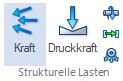
\includegraphics[scale=0.4]{figures/mechanik/Solid Edge_Strukturelle Lasten.jpg}
			\caption{Solid Edge Strukturelle Lasten}
			\label{fig:Solid Edge Strukturelle Lasten}
	\end{center}
\end{figure}


Der nächste Schritt besteht darin eine "Vernetzung" durchzuführen, um die Berechnung zu ermöglichen. Durch die Vernetzung, wird die Kontur des Bauteiles vernetzt, welche bei der Berechnung des Verhalten des Teiles auf die Kräfte, notwendig ist. 


\begin{figure} [H]
	\begin{center}
		
\includegraphics[scale=0.4]{figures/mechanik/Solid Edge_Vernetzung.jpg}
			\caption{Solid Edge Vernetzung}
			\label{fig:Solid Edge Vernetzung}
	\end{center}
\end{figure}


Mit "Berechnen", wird die Berechnung gestartet und das Ergebnis ausgegeben.
Im Ergebnis können die Verschiebung des Teiles, auftretende Spannungen und viele weitere Ergebnisse abgerufen und auch mit "Animation", animiert beobachtet und abgelesen werden. 


\begin{figure} [H]
	\begin{center}
		
\includegraphics[scale=0.4]{figures/mechanik/Solid Edge_Animation.jpg}
			\caption{Solid Edge Animation}
			\label{fig:Solid Edge Animation}
	\end{center}
\end{figure}


Die Funktion "DIN Metrische Zeichnung", kann das Bauteil in 2D Ansichten, für Zeichnungen umgewandelt werden, um das Bauteil fertigen lassen zu können. Die umgewandelten Ansichten können bemaßt und geschnitten werden, um ein bestmögliches Verständnis der Fertigungsabteilung zu versichern. Mit "Ansichtsassistent" kann das gewünschte Teil ausgewält unf umgewandelt werden.


\begin{figure} [H]
	\begin{center}
		
\includegraphics[scale=0.4]{figures/mechanik/Solid Edge_Zeichnungsansichten.jpg}
			\caption{Solid Edge Zeichnungsansichten}
			\label{fig:Solid Edge Zeichnungsansichten}
	\end{center}
\end{figure}


Mit der Funktion "DIM Metrische Baugruppe", können Einzelteile zu einem virtuellem Gerät zusammengebaut werden. Hier wird unter anderem ermöglicht Simulationen von Bewegungs- ,oder Getriebeabläufen zu erstellen. Durch die "Komponentenmontage" werden Beziehungen zwischen Teilen festgelegt und fixiert.


\begin{figure} [H]
	\begin{center}
		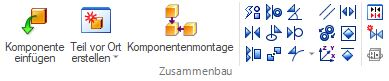
\includegraphics[scale=0.5]{figures/mechanik/Solid Edge_Zusammenbau.jpg}
			\caption{Solid Edge Zusammenbau}
			\label{fig:Solid Edge Zusammenbau}
	\end{center}
\end{figure}
>>>>>>> Stashed changes
